\documentclass{thesis}
\usepackage{graphicx}   % if you want to include graphics files
\usepackage[
    style=numeric,
    natbib=true,
    sorting=none
]{biblatex}
\usepackage{amsmath}
\usepackage{hyperref}
\usepackage{enumitem}
\usepackage{multirow}
\usepackage{adjustbox}


\makeatletter
\newcommand{\lambdabar}{{\mathchoice
  {\smash@bar\textfont\displaystyle{0.25}{1.2}\lambda}
  {\smash@bar\textfont\textstyle{0.25}{1.2}\lambda}
  {\smash@bar\scriptfont\scriptstyle{0.25}{1.2}\lambda}
  {\smash@bar\scriptscriptfont\scriptscriptstyle{0.25}{1.2}\lambda}
}}
\newcommand{\smash@bar}[4]{%
  \smash{\rlap{\raisebox{-#3\fontdimen5#10}{$\m@th#2\mkern#4mu\mathchar'26$}}}%
}
\makeatother


\addbibresource{bibliography.bib}

% Use the first command below if you want captions over 1 line indented.
% A side effect of this is to remove the use of bold for captions. 
% To restore bold, also include the second line below.
%\usepackage[hang]{caption}     % to indent subsequent lines of captions
%\renewcommand{\captionfont}{\bfseries} % only needed with caption package;
                                        %   otherwise bold is default)
                                        
%%%%%%%%%%%%%%%%%%%%  supply titlepage info  %%%%%%%%%%%%%%%%%%%%%
\thesistitle{\bf Determining Resonance Parameters of Self-Shielded Measurements in the Unresolved Resonance Region}        
\author{Alec William Golas}        
\degree{}
\department{Nuclear Engineering} % provide your area of study here; e.g.,
%  "Mechanical Engineering", "Nuclear Engineering", "Physics", etc.
\thadviser{Yaron Danon}
\signaturelines{5} 
\memberone{Dr. Wei Ji}        
\membertwo{Dr. Emily Lu}        
\memberthree{Dr. David Brown}
\memberfour{Dr. Devin Barry}
%\cothadviser{First co-adviser} %if needed
%\cocothadviser{Second co-adviser} % if needed
%  For a masters project use \projadviser instead of \thadviser, 
%  and \coprojadviser and \cocoprojadviser if needed. 
\submitdate{November 2025}        
%\copyrightyear{1685}  % if date omitted, current year is used. 
%%%%%%%%%%%%%%%%%%%%%   end titlepage info  %%%%%%%%%%%%%%%%%%%%%%
      
\begin{document} 
\titlepage             % Print titlepage   
%\copyrightpage        % optional         
\tableofcontents       % required 
\listoftables          % required if there are tables
\listoffigures         % required if there are figures


\chapter{Introduction}
\label{chap:introduction}
\section{Objective}
    The goal of this research project was to enable the determination of resonance parameters for the unresolved resonance region (URR) directly from self-shielded measurements. To accomplish this, this project involved the verification and validation of the self-shielding code SESH\cite{sesh}, which was then integrated into the nuclear resonance parameter fitting code SAMMY\cite{sammy}.


\section{Problem Description}

    In nuclear engineering, the cross section can essentially be broken up into three regions: the resolved resonance region, the unresolved resonance region, and the fast region. The resolved resonance region is where nuclear resonances can be resolved experimentally. The fast region is where we have a smooth cross section. The unresolved resonance region is where resonances cannot be resolved experimentally, but in which the resonant structure still is experimentally observed. The resonant structure in the URR is accounted for in neutron transport codes by the use of probability tables. These probability tables are essentially a histogram of different possible cross section values for any given energy. The histograms which make up these probability tables are populated by simulating cross section resonances in the URR based on average resonance parameters and the parameters' known statistical distributions. NJOY\cite{njoy} is one such code that is responsible for generating these histograms from average resonance parameters. Accounting for resonant structure is essential for correctly modeling critical systems.





    Consider the IMF-10 Criticality Benchmark\cite{icsbep}, which is a 9\% enriched cylindrical system with a depleted uranium reflector. This was modeled in MCNP using cross sections generated from the ENDF-VIII.0 nuclear data library\cite{endf-8} and processed with NJOY. In order to show the effect of the URR resonant structure, the benchmark was run once with the probability tables enabled and once with the probability tables disabled.

    \begin{table}[h!]
        \centering
        \caption{Impact of the URR on the ZPR-U9 Criticality Benchmark.}
        \begin{tabular}{|l  c  c|}
            \hline
            ~                       &   $k_{eff}$   & $\Delta \rho$ (pcm) \\
            \hline
            URR P-Tables Enabled    &   $1.00274$   & $0$ \\
            URR P-Tables Disabled   &   $0.99806$   &   $-467$ \\
            \hline
        \end{tabular}
        \label{tab:criticality-benchmark}
    \end{table}
    
    The results are given in \autoref{tab:criticality-benchmark}. In this example, the effect of accounting for URR fluctuations compared to not accounting for URR fluctuations reduced the reactivity of the system by 467 pcm. This difference in criticality is referred to as resonance self-shielding.

    While accounting for resonant fluctuations in the URR is straightforward once accurate average resonance parameters are determined, self-shielding is still going to be encountered when taking measurements in the URR. Essentially, due to the non-linearity of the cross section and the functional form of the measurements of said cross section, the average measured quantity is not equal to the measurement of the average cross section. Put more concretely, this non-equivalence can be stated as the average value of a transmission measurement is not equal to the transmission of the average cross section, or
    \begin{equation}
        \label{eq:self-shielding}
        \langle T (\sigma) \rangle \neq T(\langle \sigma \rangle)
    \end{equation}
    in which $\langle ... \rangle$ represents a quantity averaged over some energy region.
    
    This issue is shown in \autoref{fig:self-shielding-demo}, using \textsuperscript{181}Ta as an example. Here, the transmission of a 0.105 at/barn thick sample is simulated in three ways. First, in which the $\sigma(E)$ was finely resolved, such that a true $T(E)$ was obtained. Second, in which the transmission is obtained as an energy-averaged quantity, $\langle T \rangle$. Finally, the energy-average of the known cross section $\langle \sigma \rangle$ was obtained over the same energy region and the ``transmission of the average cross section'' was calculated, $e^{-n \langle \sigma \rangle}$. The two average quantities, $\langle T\rangle$ and $e^{-n \langle \sigma \rangle}$, not being equal is exactly what prevents the use of a nuclear fitting code like SAMMY\cite{sammy} to be used with URR measurements that have not accounted for self-shielding.

    \begin{figure}
        \centering
        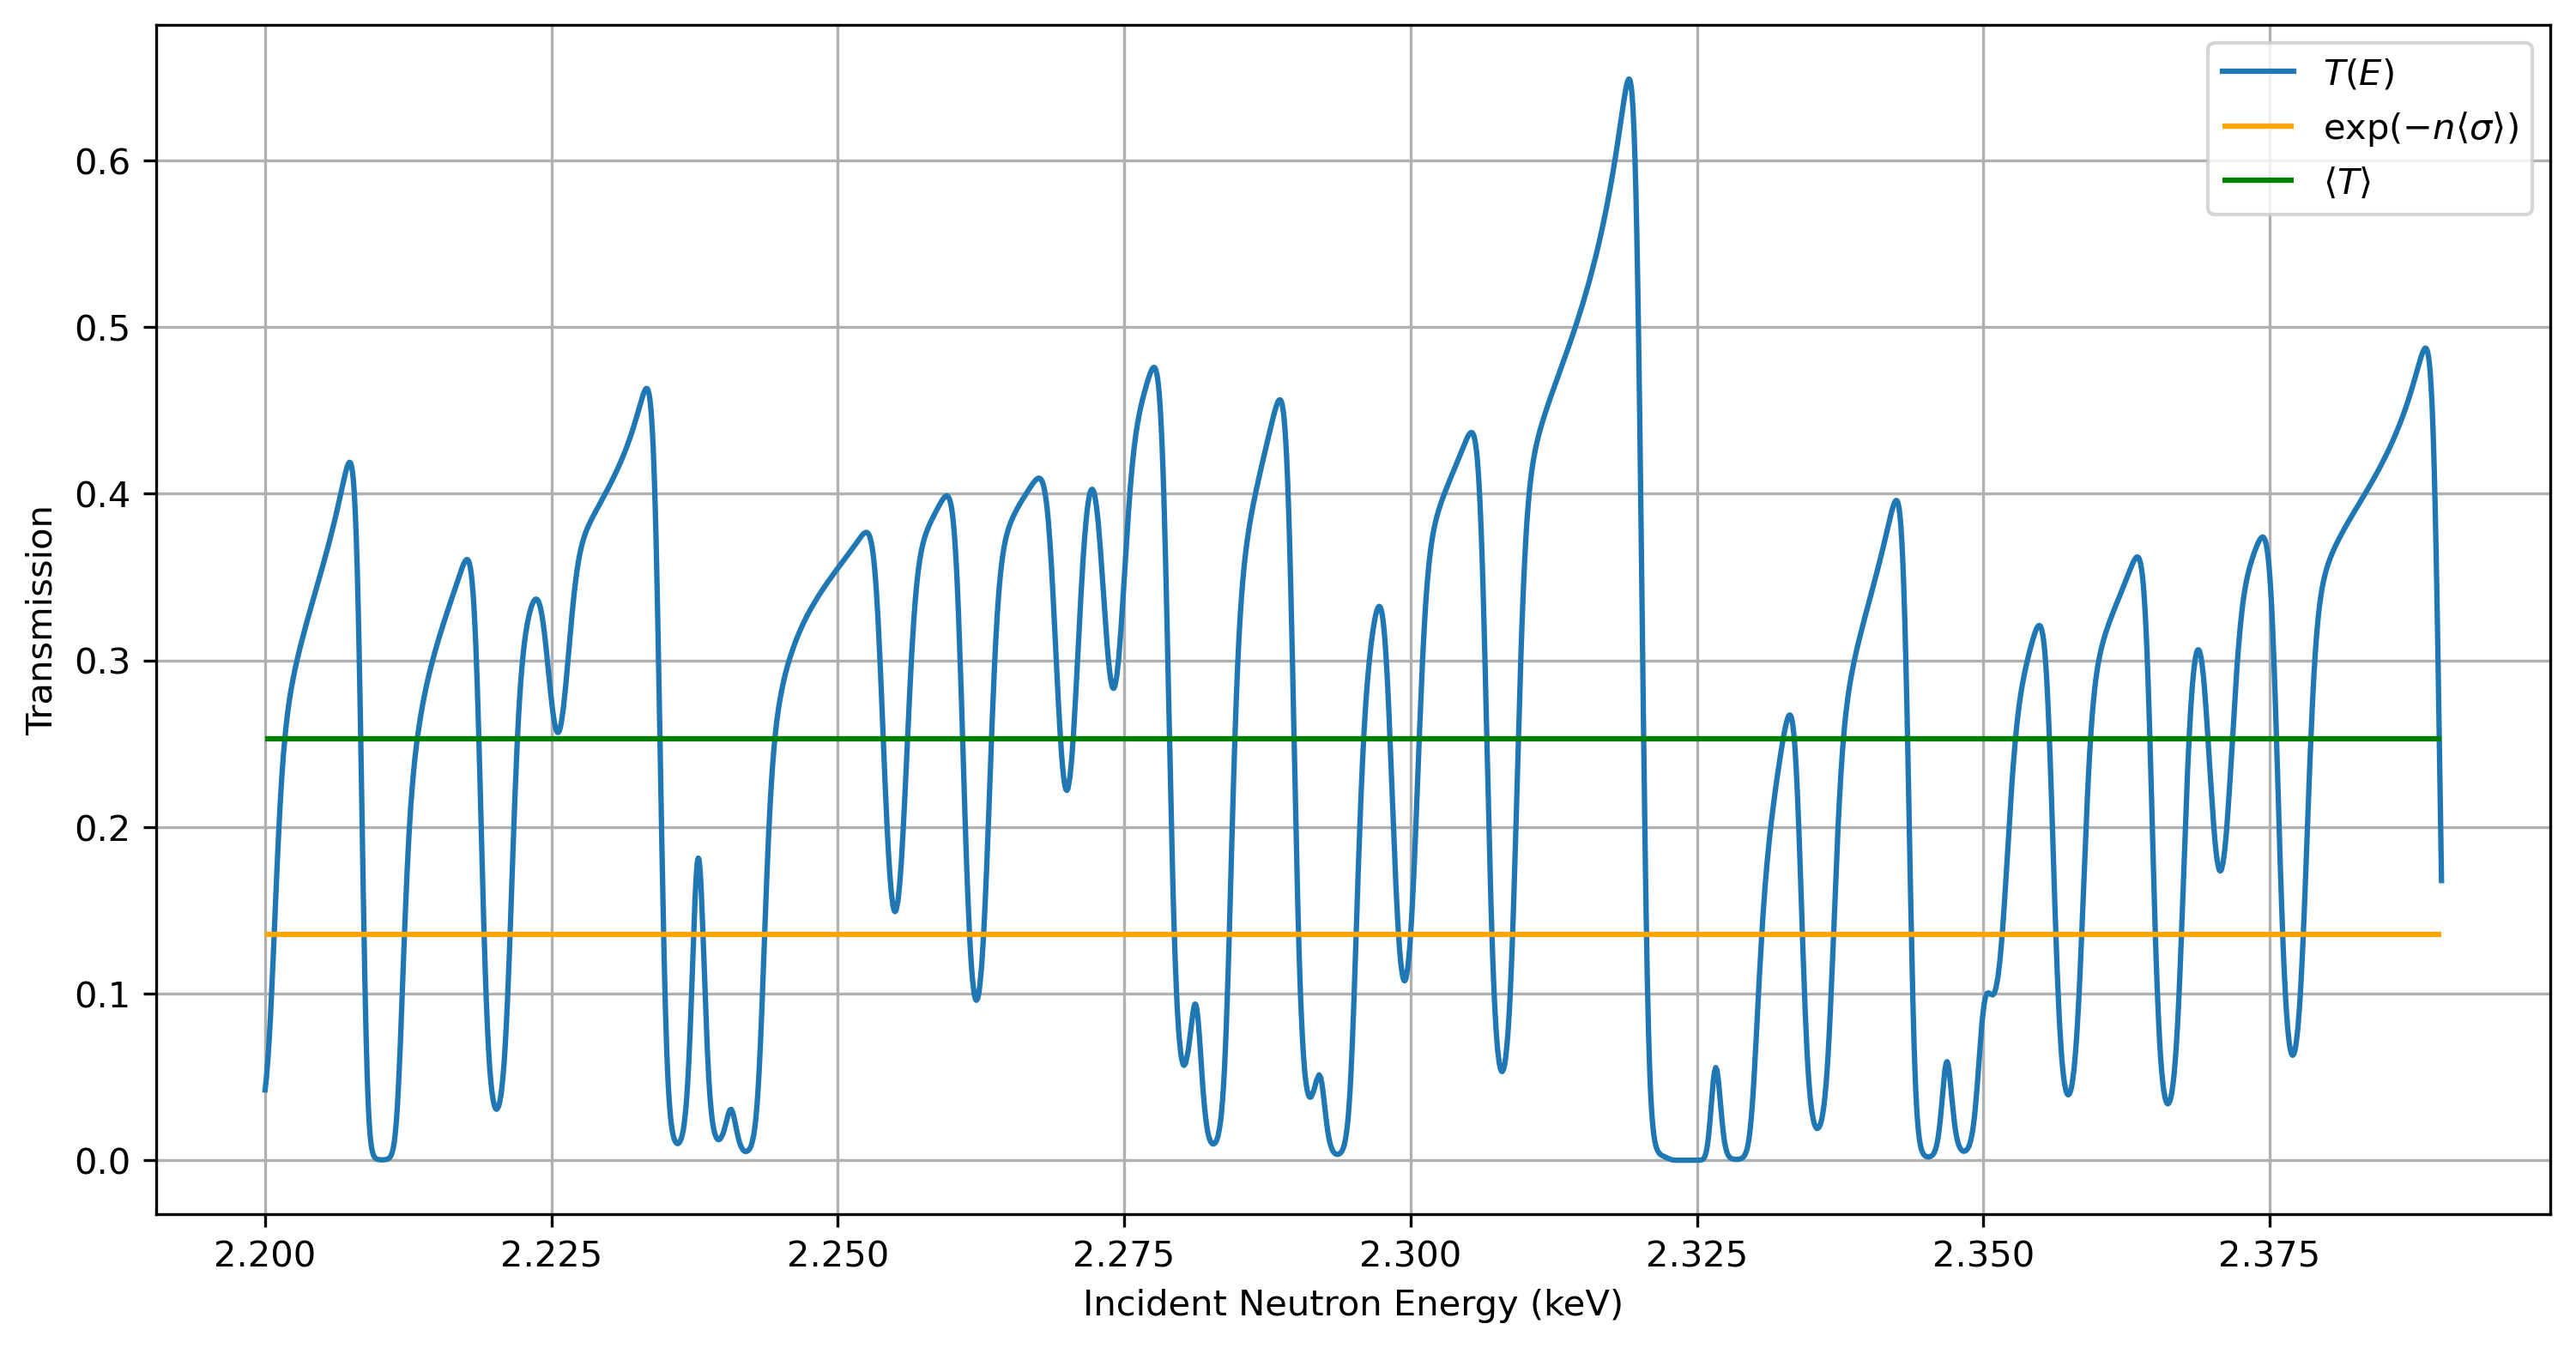
\includegraphics[width=0.95\textwidth]{Introduction/Figures/transmission-example.png}
        \caption{Demonstration of Self-Shielding for \textsuperscript{181}Ta comparing the `True Transmission' (blue line), `Average Transmission' (green line), and `Transmission of Average Cross Section' (orange line).}
        \label{fig:self-shielding-demo}
    \end{figure}

    To summarize, three facts are true:
    \begin{enumerate}
        \item The resonant structure in the URR cannot be ignored in modeling critical systems.
        \item Modeling the resonant structure in the URR requires accurate resonance parameters.
        \item URR parameters cannot be directly determined from transmission and capture experiments due to self-shielding.
    \end{enumerate}

    Therefore, a problem remains: how can an average measurement be expressed as a function of the average cross section? It wouldn't be sufficient to fit resonance parameters using the ``uncorrected'' cross-section, i.e.,
    \begin{equation}
        \overline{\sigma} = -\frac{1}{n} \ln{\langle T \rangle}
    \end{equation}
    as this value is heavily dependent on experimental conditions such as temperature and sample thickness, and does not account for self-shielding. The resonance parameters obtained from fitting $\overline{\sigma}$ would not accurately represent the true cross section.

    If resonance parameters which accurately describe the true average cross section are to be obtained, self-shielding must be accounted for. In order to do that, a correction factor is used, such that
    \begin{equation}
        \label{eq:self-shielded-transmission}
        \langle T \rangle = e^{-n \langle \sigma \rangle} C_T
    \end{equation}
    This `transmission correction factor', $C_T$, corrects for the self-shielding effect produced by the resonant fluctuations in the URR.

    This project integrated self-shielding correction factors directly into SAMMY, enabling the code to fit self-shielded URR transmission and capture yield measurements. Additionally, the capability to fit multiple isotope samples, such as self-shielded transmission and capture measurements of natural samples, was introduced: a feature not previously available in SAMMY's URR fitting. This new functionality significantly modernized SAMMY's URR fitting interface. This developed package was then applied to a new evaluation of the unresolved resonance region for Zr\textsuperscript{90} and Zr\textsuperscript{91}, utilizing natural datasets to improve the performance of the fit, which had been previously impossible due to the lack of multi-isotope functionality.

\chapter{Statistical Theory of the Unresolved Resonance Region}
\label{chap:theory}
\section{Unresolved Resonance Region}
\label{sec:unresolved-resonance-region}

The Unresolved Resonance Region (URR) presents similar nuclear reaction phenomena as the Resolved Resonance Region (RRR); however, the crucial distinction lies in the experimental observability of individual resonances. In the URR, the resonances are too closely spaced in energy to be experimentally resolved, meaning that individual resonance parameters (e.g., resonance energies and widths) cannot be directly determined. This stands in contrast to the RRR, where the Single-Level Breit-Wigner (SLBW) approximation (or more complex multi-level formulations) can precisely describe the energy-dependent cross section based on discrete resonance parameters.

Because a complete set of individual resonances cannot be resolved, it becomes impractical and often impossible to calculate the "true" point-wise cross section in the URR. Therefore, instead of determining explicit resonance shapes, evaluators resort to calculating \textit{average} cross sections. These average cross sections are derived from statistical properties of the resonances, such as average level spacings and average resonance widths, rather than their individual values. This approach assumes that these parameters are sufficiently statistical and therefore accurately models the average cross section in the URR.

This formulation provides a convenient analytical form for the average total cross-section. However, it is missing a crucial element of the unresolved resonance region. The underlying statistical nature of the \textit{true} cross section in the unresolved resonance region exhibits significant rapid fluctuations around this analytical average cross section. These rapid fluctuations are responsible for resonant self-shielding. Resonant self-shielding significantly impacts transport equations, and must be accounted for to accurately model neutron transport. The following section characterizes the impact of cross section variance due to resonance fluctuations.

\section{Resonance Self Shielding}
\label{sec:resonance-self-shielding}
Resonance self-shielding is a phenomena which occurs when the resolution of a measurement is less than the level spacing between resonances. It can be summarized as the non-linear relationship between an observable quantity, i.e., transmission, and the total cross-section. Self-shielding is a consequence of the variance of the cross-section over some energy region. As the variance in the cross-section increases, the energy-averaged transmission increases relative to the transmission of the average cross-section,
\begin{equation}
    \label{eq:self-shielding-definition}
    \langle T \rangle > e^{-n \langle \sigma \rangle}
\end{equation}
in which the operator $\langle \cdot \rangle$ denotes an energy-averaged quantity,
\begin{equation}
    \label{eq:energy-average-operator}
    \langle \cdot \rangle = \frac{1}{E_{1} - E_{0}} \int_{E_{0}}^{E_{1}} \cdot dE
\end{equation}

The energy-averaged transmission, $\langle T \rangle$, is given by:
\begin{equation}
    \label{eq:energy-average-Transmission}
    \langle T \rangle = \langle e^{-n \sigma(E)} \rangle
\end{equation}
in which $\sigma(E)$ is the total cross-section as a function, and $n$ is the thickness of some material.

To demonstrate how the variance in the cross-section contributes to self-shielding, consider the Taylor-Series expansion of $\langle T \rangle$. The energy-differential transmission can be redefined in terms of the average cross-section over that energy bin, and the deviation of the energy-differential cross-section from the average:
\begin{equation}
    \left\langle e^{-n \sigma(E)} \right\rangle = \left\langle e^{-n \langle \sigma \rangle} e^{-n \left(\sigma(E) - \langle \sigma \rangle \right)} \right\rangle
\end{equation}

Because $\langle \sigma \rangle$ has to be constant over that energy region, that can be rearranged to:
\begin{equation}
    \label{eq:taylor-series-step}
    \left\langle e^{-n \sigma(E)} \right\rangle = e^{-n \langle \sigma \rangle} \left\langle e^{-n \left( \sigma(E) - \langle \sigma \rangle \right)} \right\rangle
\end{equation}

The second term in \autoref{eq:taylor-series-step} can be approximated using a Taylor expansion:
\begin{equation}
    e^{-n \left( \sigma(E) - \langle \sigma \rangle \right)} \approx 1 + n (\sigma(E) - \langle \sigma \rangle) + \frac{n^{2}}{2} (\sigma(E) - \langle \sigma \rangle)^2
\end{equation}
Taking the average of this approximation, and noting that $\langle \sigma(E) - \langle \sigma \rangle \rangle = 0$, we get:
\begin{equation}
    \left\langle e^{-n \left( \sigma(E) - \langle \sigma \rangle \right)} \right\rangle \approx 1 + \frac{n^{2}}{2} \langle (\sigma(E) - \langle \sigma \rangle)^2 \rangle = 1 + \frac{n^{2}}{2} \text{Var}(\sigma)
\end{equation}
This leads to the final approximation for $\langle T \rangle$:
\begin{equation}
    \label{eq:taylor-series-expansion}
    \langle T \rangle \approx e^{-n \langle \sigma \rangle} \left(1 + \frac{n^{2}}{2} \text{Var}(\sigma) \right) = e^{-n \langle \sigma \rangle} + \frac{n^{2}}{2} e^{-n \langle \sigma \rangle} \text{Var}(\sigma)
\end{equation}

Clearly, according to \autoref{eq:taylor-series-expansion}, as the variance in the cross-section increases, the self-shielding will increase.

\section{The Self-Shielding Correction Factor}
\label{sec:correction-factor}

The self-shielding correction factor is used to solve the inequality given in \autoref{eq:self-shielding-definition}. It is defined as:
\begin{equation}
    C_{T} = \frac{\langle e^{-n \sigma (E)} \rangle}{ e ^{- n \langle \sigma \rangle}}
\end{equation}

The experimental transmission obtained in the unresolved resonance region, $\langle T \rangle$, is given by:
\begin{equation}
    \label{eq:transmission}
    \left\langle T \right\rangle = \frac{1}{E_2 - E_1} \int_{E_1}^{E_2} e^{-n \sigma(E)}dE
\end{equation}
in which $\sigma(E)$ is the true cross section of the material. It is assumed that the energy bin is wide enough such that a statistically meaningful sample of resonances are captured.

In order to express the average transmission as a function of the average cross section:
\begin{equation}
    \label{eq:transmission-of-average}
    \left\langle T \right\rangle = \frac{1}{E_2 - E_1} \int_{E_1}^{E_2} e^{-n \left( \sigma(E) + \langle \sigma \rangle - \langle \sigma \rangle \right)}dE
\end{equation}
in which 
\begin{equation}
    \label{eq:energy-average-cross-section}
    \left\langle \sigma \right\rangle = \frac{1}{E_2 - E_1} \int_{E_1}^{E_2} \sigma(E) dE
\end{equation}
Therefore, the term defining the ``transmission of the average cross section'', $e^{-n \langle \sigma \rangle}$, can be removed, such that 
\begin{equation}
    \label{eq:corrected-average-transmission}
    \langle T \rangle = e^{-n \langle \sigma \rangle} C_T
\end{equation}
in which the term $C_T$ is known as the transmission correction factor, and is defined as:
\begin{equation}
    \label{eq:transmission-correction-factor}
    C_T = \frac{1}{E_2 - E_1} \int_{E_1}^{E_2} e^{-n \left( \sigma(E) - \langle \sigma \rangle \right)}dE
\end{equation}

In other words, the correction factor is the average deviation of the true cross section from the mean cross section over a given energy bin.
\begin{equation}
    \label{eq:ct-elegant-form}
    C_T = \left\langle e^{-n (\sigma - \langle \sigma \rangle)} \right\rangle
\end{equation}
or in a form that will be more useful in a later section (e.g. \autoref{sec:sesh}),
\begin{equation}
    \label{eq:ct-sesh-form}
    C_T = \frac{\langle e^{-n \sigma} \rangle}{ e^{-n \langle \sigma \rangle}}
\end{equation}


It should be noted that this is specifically the \textit{transmission} self-shielding correction factor. Other forms will be used later, but the end goal is the same: determine the average measurement as a function of the average cross section.

\section{Sampling Cross Sections from Average Parameters}
\label{sec:mc-sampling-from-average-parameters}

As previously stated in \autoref{sec:resonance-self-shielding}, in the Unresolved Resonance Region, individual resonances cannot be directly observed due to their close spacing. As such, only average resonance parameters can be obtained from measurements in the URR. While analytical equations, (e.g., \autoref{eq:hauser-feshbach-cross-section}), provide energy-averaged cross sections based on these average parameters, these analytical solutions intrinsically yield only the average behavior. They do not, however, directly provide the variance of the true, fluctuating energy-dependent cross section within the URR. The phenomenon of resonance self-shielding (discussed in \autoref{sec:resonance-self-shielding}) is directly dependent on this variance. However, this only discusses the determination of self-shielding from a known energy differential cross-section, which is not able to be observed.

Since the true energy-differential cross section in the URR is unknown, and its variance cannot be directly calculated from the average parameters alone, Monte Carlo methods provide the necessary means to address this challenge. By statistically sampling individual resonance parameters from their known probability distributions, Monte Carlo sampling allow for the generation of distribution of cross section "realizations" which agree with the average analytical cross section and account for the variance in cross section around said average. This section will detail how these fluctuating cross sections are determined from average parameters by leveraging the Single-Level Breit-Wigner (SLBW) equation, and sampling parameters from their respective statistical distributions.

\subsection{The Single-Level Breit-Wigner (SLBW) Equation for Cross Section Reconstruction}
\label{sec:slbw-for-sampling}

The Single-Level Breit-Wigner (SLBW) approximation, typically used in the Resolved Resonance Region (RRR) for well-separated resonances, serves as the fundamental basis for reconstructing cross-section distributions from sampled resonance parameters in the URR. For a given channel $c$, the total SLBW cross section is determined as a sum over resonances $r$ via:
\begin{equation}
    \label{eq:slbw}
    \sigma_c = \frac{ 4 \pi g_c}{k_c^2} \sum_r 
        \left\{ \sin^2{\phi_c} + \frac{\Gamma_{n,r,c}}{\Gamma_{tot,r,c}}
            \left( \psi \cos{2 \phi_c} + \chi \sin{2\phi_c}
            \right)
        \right\}
\end{equation}
The incoming channel $c$ corresponds to a unique combination of $J,\ell,\pi$ quantum numbers. The statistical spin factor, $g_c$ is defined as
\begin{equation}
    g_c = \frac{2J + 1}{2(2I + 1)}
\end{equation}
in which $I$ is the spin of the target nucleus, and $J$ is the spin associated with channel $c$. $\phi_c$ is the hard-sphere scattering phase shift of a particular channel\cite{t2}.

$\psi$ and $\chi$ are the Doppler broadened resonance profiles. Those are determined by using the Faddeeva function\cite{algo-916}, such that
\begin{equation}
    \label{eq:faddeeva}
    \psi + i\chi = \frac{\sqrt{\pi}}{2}\theta w \left(\frac{\theta x}{2}, \frac{\theta}{2} \right)
\end{equation}
in which $\theta$ is the Doppler width,
\begin{equation}
    \theta = \frac{\Gamma_{tot}}{\sqrt{\frac{4 \kappa T E}{A}}}
    \label{eq:doppler-width}
\end{equation}
$x$ is the resonance shape,
\begin{equation}
    x = \frac{2 (E - E_r)}{\Gamma_{tot}}
\end{equation}
and $w(\alpha,\beta)$ is defined as
\begin{equation}
    w(\alpha,\beta) = \frac{i}{\pi} \int_{-\infty}^{\infty} \frac{e^{-t^2}}{\alpha + i\beta - t}dt
\end{equation}

The total microscopic cross section for a given nuclide at a specific energy is then determined by summing the contributions from all possible incoming channels $c$. Each channel corresponds to a unique set of quantum numbers (spin, orbital angular momentum, and parity) that contribute to the reaction. The detailed determination of all possible channel states will be elaborated in a later section. It is crucial to note that this SLBW formulation, as presented, presumes that the individual resonance parameters ($E_r$, $\Gamma_{n,r}$, and $\Gamma_{tot,r}$, for each resonance $r$) are precisely known. However, in the URR, these individual parameters are not experimentally resolved. Instead, only their \textit{average} values and statistical distributions are known. This discrepancy necessitates the use of statistical sampling techniques to generate instances of these resonance parameters from their average values and distributions, which then allows for the reconstruction of fluctuating cross sections using the SLBW equation.

\subsection{Sampling Cross-Sections from Average Parameters}
\label{sec:sampling-parameters}


The procedure for generating a statistical realization of the cross section over a given energy range involves several steps, iterated across different channels and multiple times to build a comprehensive distribution. For each given channel $c$, defined by a unique $(\ell, J, \pi)$ combination, a ladder of resonance energies is determined. This is done by sampling from the Wigner Distribution, in which
\begin{equation}
    P(s) = \frac{s\pi}{2 \langle D \rangle_c^2} e^{-\frac{\pi s^2}{4 \langle D \rangle_c^2}}
\end{equation}
where $\langle D \rangle_c$ is the average level spacing associated with that channel $c$, and $s$ is the sampled level spacing. This is used to produce a resonance ladder
\begin{equation}
    E_{c,r+1} = E_{c,r} + s
\end{equation}

The following step is to sample neutron widths for each channel and resonance energy.

\begin{equation}
    \Gamma_{n,r,c} = P\left( \frac{\Gamma_{n,c}^0}{\langle \Gamma_{n,c}^0  \rangle}\right)\langle \Gamma_{n,c}^0  \rangle \nu_c(E_r) \sqrt{E_r}
\end{equation}
in which $\langle \Gamma_{n,c}^0  \rangle$ is the reduced neutron width, $\nu_c$ is the penetrability of channel $c$, and $P\left( \Gamma_{n,c}^0 / \langle \Gamma_{n,c}^0  \rangle \right)$ is the Porter-Thomas distribution, where:
\begin{equation}
    P(x) = \frac{e^{-x/2}}{\sqrt{2\pi x}}
\end{equation}

The total resonance width is determined as a sum over the neutron width plus the other possible channels, i.e., radiation width and fission width:
\begin{equation}
    \Gamma_{tot,r,c} = \Gamma_{n,r,c} + \Gamma_{\gamma,r,c} + \Gamma_{f,r,c}
\end{equation}

These sampled parameters are processed via the steps described in \autoref{sec:slbw-for-sampling} to be input into \autoref{eq:slbw} and generate a cross section for that given channel $c$. This process is repeated for all possible channels to provides a single realization of the total cross section for a given set of average parameters:
\begin{equation}
    \sigma_{tot}^i = \sum_c \sigma_c
\end{equation}
Finally, this is repeated some $N$ number of realizations to produce a population of sampled cross sections, $\{ \sigma_{tot}^1, \sigma_{tot}^2, \ldots, \sigma_{tot}^{N} \}$. This set of sampled cross sections, if defined using accurate average parameters over some statistical number of resonances, will accurately reproduce the true variance in the energy-differential cross section over some energy bin.

This is the general procedure of how nuclear data processing codes (NJOY, FRENDY, AMPX) account for self-shielding in the URR. Self-shielding due to cross section variance from resonant fluctuations can therefore be accurately modeled strictly from average parameters.

Note, this only addresses total cross section. It does not mention partial cross sections, interpreting between parameters to be used in \autoref{eq:hauser-feshbach-cross-section} and \autoref{eq:slbw}, energy dependencies, or any approximations. Those details are implementation-specific, and will be discussed in subsequent chapters.


\chapter{Implementation Details}
\label{chap:implementation}
This section describes the implementation of SESH into SAMMY as required for fitting resonance parameters to self-shielded URR measurements.

\section{URR Representation in SAMMY}

The average cross section in the URR is typically defined according to Hauser-Feshbach theory, which provides a framework for describing nuclear reactions proceeding through a compound nucleus when many channels are open and individual resonance effects are smeared out. The energy-averaged total cross section for an incoming channel $c$ can be expressed as:

\begin{equation}
    \label{eq:hauser-feshbach-cross-section}
    \langle \sigma_c \rangle =
    2 \pi \lambdabar_c^2 g_c \left\{
    1 - \frac{
            \cos{ ( 2 \phi_c)} \left[
                1 - \pi^2P_c^2 s_c^2 -  \left( P_c R_c^\infty \right)^2
            \right]
            + \sin{(2 \phi_c)} 2 P_c R_c^\infty
        }{
            \left( 1 + \pi P_c s_c \right)^2 + \left( P_c R_c^\infty \right)^2
    }
    \right\} \quad \text{}
\end{equation}
In this formulation, $\lambdabar$ is the reduced de Broglie wavelength for the neutron, $g_c$ is the statistical spin factor defined as $g_c = \frac{2J + 1}{2(2I + 1)}$ where $I$ is the spin of the target nucleus , and $\phi_c$ is the hard-sphere scattering phase shift for a particular channel. The form of $\phi_c$ depends on the orbital momentum $\ell$ and is a function of $\rho = \frac{a_c}{\lambdabar}$, where $a_c$ is the scattering radius of the target nucleus.

The parameters of significance to transmission self-shielding in the URR, which distinguish this average cross section from a simple energy average of RRR cross sections, are the distant level parameter $R^\infty_c$ and the strength function $\Tilde{S}_c$. Here, $P_c$ is the neutron penetrability, and $s_c$ is the pole strength, defined as $s_c = \Tilde{S}_c\lambdabar a_c \sqrt{E}/2$. The strength function $\Tilde{S}_c$ characterizes the average reduced width of resonances for a given orbital $\ell$.


\section{Converting from SAMMY Parameters to SESH Parameters}
    \subsection{Calculating Available Channels}

    As mentioned in the previous section, the relevant URR parameters are all given only as their $\ell$ basis. As a requirement for simulating resonances for calculating resonance self-shielding, these parameters need to be calculated according to $(J,\ell,\pi)$ rather than just $\ell$ dependencies.

    For an isotope with a ground-state spin $I$ interacting with a neutron (which has an intrinsic spin of $s_n = 1/2$), there are two possible channel spins: $s_{-} = I - 1/2$ and $s_{+} = I + 1/2$. This leads to two separate cases for the total angular momentum $J$: one for $s_{-}$ and one for $s_{+}$:
    \begin{align}
        J_{-} &= \left\{ \left|s_{-} - \ell\right|, \left|s_{-} - \ell\right| + 1, \cdots, s_{-} + \ell \right\}\\
        J_{+} &= \left\{ \left|s_{+} - \ell\right|, \left|s_{+} - \ell\right| + 1, \cdots, s_{+} + \ell \right\}
    \end{align}
    One common assumption is that spin-group parameters are assumed to be independent of parity, i.e., $(J, \ell, -1) = (J, \ell +1)$. As a consequence, only $J$ and $\ell$ need to be considered when calculating resonances. Instead, the important factor to consider is the degrees of freedom, or the multiplicity, $\mu$. If the same $J,\ell$ combination can be calculated from $s_{+}$ and $s_{-}$ channel spins, then $\mu_i = 2$. Otherwise, $\mu_i=1$.

    \begin{equation}
        \begin{array}{rrrrrrrr}
J_{-}: & \{ & \left|s_{-} - \ell\right|, & \left|s_{-} - \ell\right| + 1, & \dots, & s_{-} + \ell ~ & & \} \\
J_{+}: & \{ & & \left|s_{+} - \ell\right|, & \dots, & s_{+} + \ell-1, & s_{+} + \ell & \} \\[1em] \hline \\[-0.5em]
\mu_J: & \{& 1, & 2, & \dots, & 2, & 1 & \} \\
\end{array}
    \end{equation}

    \subsection{Converting from $R^\infty$ to $R'$}

    \subsection{Converting Inelastic Strength to Inelastic Widths from Channels}

\section{Improving Level Density Energy Dependency}

\section{Doppler Broadening Bug}
    The primary cause of the disagreement was determined to be the result of an error in the Doppler broadening subroutine that was originally present in SESH. In order to perform the Doppler broadening, the complex error function, also known as the Faddeeva function, is utilized. The issue was in the original algorithm, in cases where $\beta$ was less than 0.01. Recall that
    \begin{equation}
        w(\alpha,\beta) = \frac{i}{\pi} \int_{-\infty}^{\infty} \frac{e^{-t^2}}{\alpha + i\beta - t}dt
    \end{equation}
    and
    \begin{equation}
        \beta = \frac{\theta}{2} = \frac{\Gamma_{tot}}{4\sqrt{\frac{ \kappa T E}{A}}}
        \label{eq:doppler-beta}
    \end{equation}

    In instances where $\beta \leq 0.01$, the algorithm would incorrectly return the 0 Kelvin value for the $\psi$ parameter, shown in \autoref{fig:beta-error}.
    \begin{figure}
        \centering
        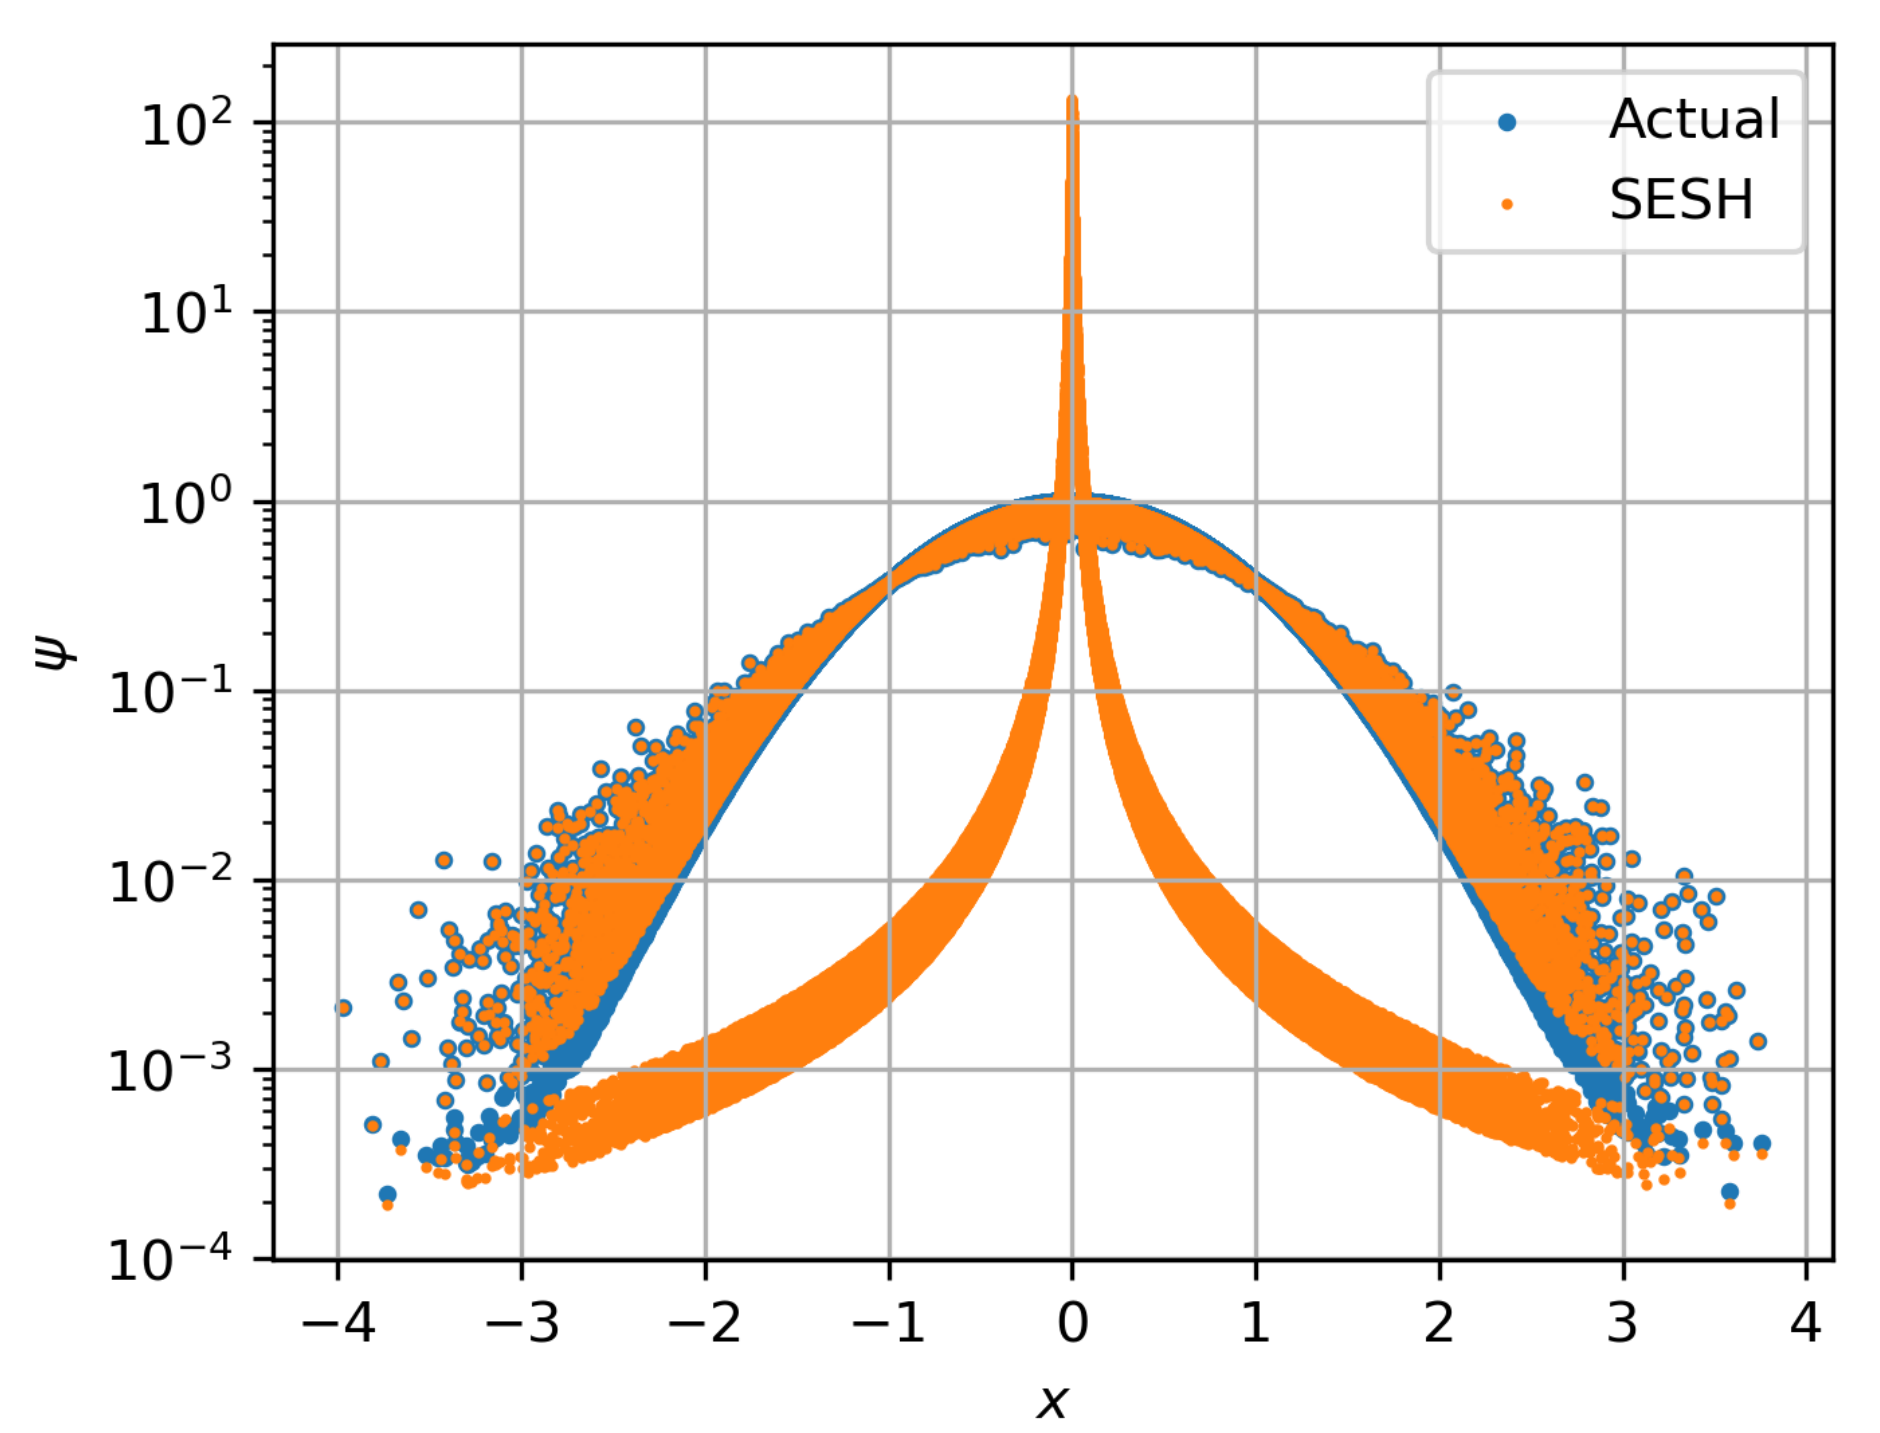
\includegraphics[width=0.95\linewidth]{Implementation/Figures/beta-error.png}
        \caption{Comparing results of SESH's Faddeeva function output with what the Faddeeva function actually calculates given the same inputs.}
        \label{fig:beta-error}
    \end{figure}
    
    One significant effect of this bug is due to the inverse relationship between $\beta$ and energy, shown in \autoref{eq:doppler-beta}. As the energy of the incident neutron increases, the probability of $\beta$ being sampled as less than 0.01 increases. Consequently, as energy increases, the probability of the 0 Kelvin cross section being returned also increased.

\section{Energy Deposition Improvement}
    Originally in SESH, there was a very simple approximation for sampling what energy an interaction occurred at. It was assumed that every neutron lost the average scattering energy per collision, independent of scattering angle, i.e.,
    \begin{equation}
        E' = E \left[ 1 - \frac{2A}{\left( 1 + A \right)^2} \right]
    \end{equation}
    for all post-collision neutrons. This enabled all of the energy dependent parameters that did not get sampled using the Monte Carlo method to be pre-calculated efficiently. However, it was assumed this would be an insufficient approximation for thick samples in which many collisions were expected.
    
    This was substituted with an angle-dependent energy sampling procedure. The scattering angle of each post collision neutron would be sampled assuming an isotropic scattering distribution, and the post collision energy would be calculated as a function of the scattering angle,
    \begin{equation}
        E' = E \frac{A^2 + 2 A \mu_c + 1}{\left( A + 1 \right)^2}
    \end{equation}
    in which
    \begin{equation}
        \mu_c = \cos\phi_c
    \end{equation}
    where $\phi_c$ is the exit angle of the post-collision neutron in the center-of-mass system.
    \begin{figure}
        \centering
        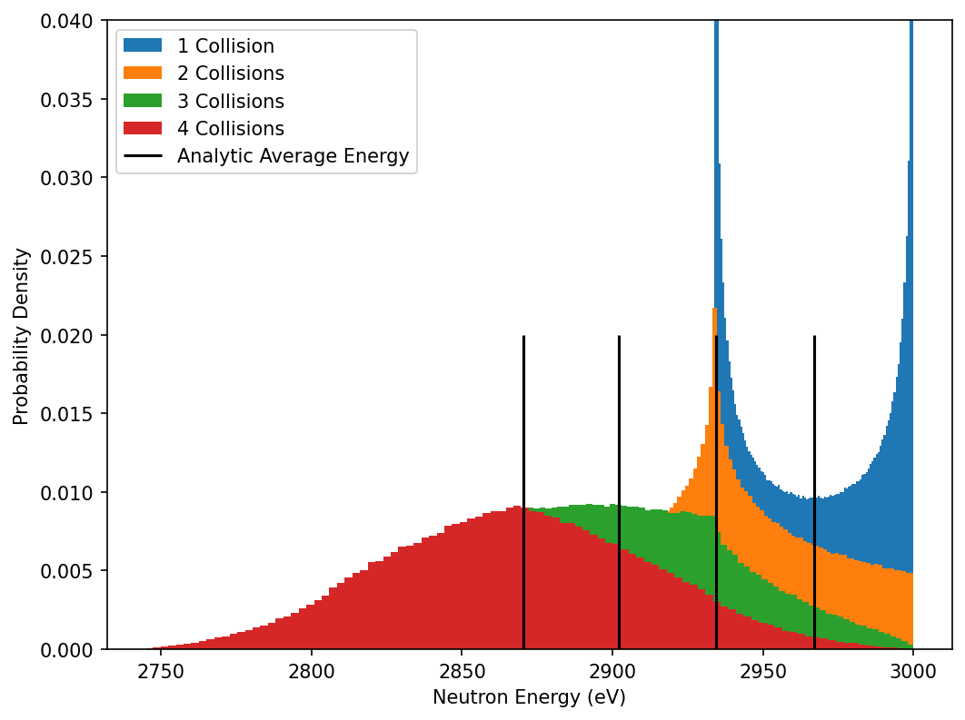
\includegraphics[width=0.95\linewidth]{Implementation/Figures/multiple_scattering.png}
        \caption{Distribution of neutrons after each collision using the old SESH post-collision energy sampling method and the new angle-dependent sampling in a 12mm \textsuperscript{181}Ta sample at 3keV initial incident energy.}
        \label{fig:multiple-scattering}
    \end{figure}

% \chapter{Transmission Correction}
% \label{chap:transmission-correction}
% \input{Transmission Correction/transmission-correction}

\chapter{Capture Yield Correction}
\label{chap:capture-yield-correction}
Another important quantity to correct for in the unresolved resonance region is capture yield. In these experiments, there are two phenomena at play: first the resonance self shielding, as described in \autoref{sec:resonance-self-shielding}. The second effect is called multiple scattering.

\section{Multiple Scattering in a Cylindrical Sample}
\label{sec:multiple-scattering}

Multiple scattering is an effect which occurs in which a neutron is scattered one or more times before being captured in a sample. As the thickness of the sample increases, the probability of a scattered neutron experiencing a subsequent reaction (that being a capture or additional scattering events) also increases. Therefore, neutrons which undergo scattering events can end up miscounted as captures, artificially increasing the measured yield.
\begin{figure}[H]
    \centering
    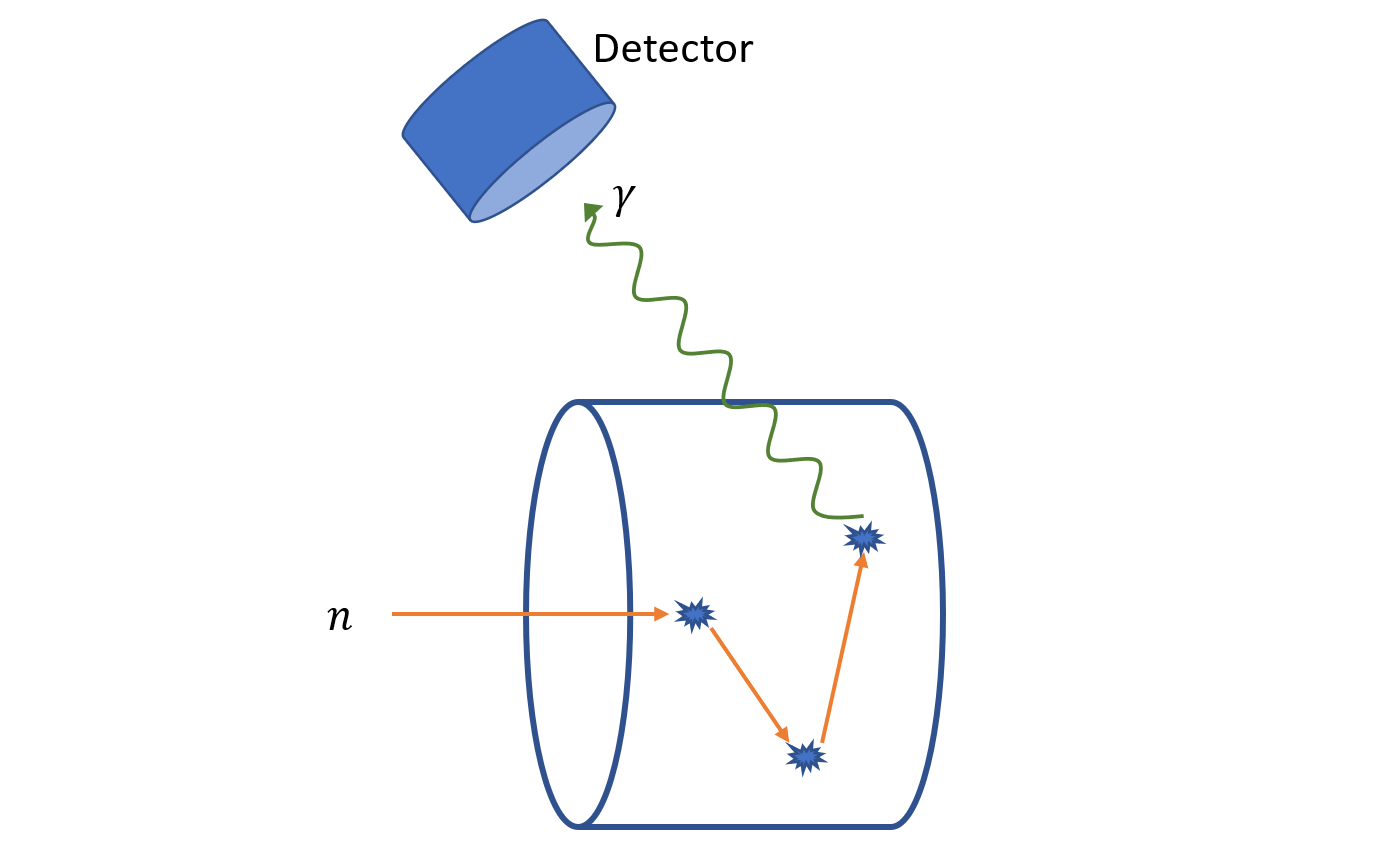
\includegraphics[width=0.75\linewidth]{Capture Yield/Figures/multiplescattering.png}
    \caption{Illustration of a neutron undergoing multiple scattering events, and getting miscounted as a capture event.}
    \label{fig:multiple-scattering-example}
\end{figure}
This is illustrated in \autoref{fig:multiple-scattering-example}, in which a neutron scatters twice before being captured.

This correction is made with reference to the thin sample approximation,
\begin{equation}
    \label{eq:thin-sample-approximation}
    \left\langle Y \right\rangle \approx n \left\langle \sigma_\gamma \right\rangle 
\end{equation}
where $\left\langle Y \right\rangle$ is the average yield, $n$ is the sample thickness, and $\left\langle \sigma_\gamma \right\rangle$ is the average capture cross section. The capture correction $C_C$ corrects the thin sample approximation such that
\begin{equation}
    \label{eq:correction-thin-sample-approximation}
    \left\langle Y \right\rangle = n \left\langle \sigma_\gamma \right\rangle C_C
\end{equation}

In order to calculate the correction, a series of Monte Carlo simulations are used to simulate a neutron undergoing a series of capture or scattering events in a cylindrical disc target. The target has a radius $R$, is parallel to the $z$ axis, and with front and rear faces located at $z=0$ and $z=n$, respectively, which are centered at $(x,y)=(0,0)$. A neutron is born at the energy of interest, $E^0$, and is incident on the front face of the target, with the location
\begin{equation}
    \label{eq:incident-neutron-location}
    \overrightarrow{x}^0 = \begin{bmatrix}
        x^0 \\
        y^0 \\
        z^0
    \end{bmatrix} =
    \begin{bmatrix} 
        r_0\cos{\left( \theta_0 \right)} \\
        r_0\sin{\left( \theta_0 \right)} \\
        0
    \end{bmatrix}
\end{equation}
where
\begin{align*}
    r_0 &= R\sqrt{\zeta}, \\
    \theta_0 &= 2\pi\zeta,
\end{align*}
and $\zeta$ is a uniformly distributed random value between 0 and 1. The neutron is also traveling along the $z$-axis, and therefore is born with the direction vector
\begin{equation}
    \label{eq:incident-neutron-location}
    \overrightarrow{\Omega}^0 = \begin{bmatrix}
        \Omega^0_u \\
        \Omega^0_v \\
        \Omega^0_w
    \end{bmatrix} =
    \begin{bmatrix}
        0 \\
        0 \\
        1
    \end{bmatrix}
\end{equation}

Cross sections are sampled at the energy $E^0$ according to the procedure described in \autoref{sec:mc-sampling-from-average-parameters}. These values are then used to produce the average cross-sections,
\begin{align}
    \label{eq:average-total-cross-section}
    \overline{ \sigma_{t} }^{0} &= \sum_{j} \sigma_{t,j}^{0} \delta_{j} \\
    \label{eq:average-capture-cross-section}
    \overline{ \sigma_{\gamma} }^{0} &= \sum_{j} \sigma_{\gamma,j}^{0} \delta_{j} \\
    \label{eq:average-scattering-cross-section}
    \overline{ \sigma_{sc} }^{0} &= \sum_{j} \sigma_{sc,j}^{0} \delta_{j}
\end{align}
where $\overline{ \sigma_{t} }$, $\overline{ \sigma_{\gamma} }$, and $\overline{ \sigma_{sc} }$  are the weighted average total, capture, and scattering cross-sections respectively. The $0$ superscript indicates that the cross-sections are taken at the energy $E^{0}$, i.e., before any scattering events have occurred. The terms $\sigma_{j}^0$ and $\delta_{j}$ are the microscopic cross-section and relative abundance of the $j^{th}$ isotope, respectively.

\section{Scattering Events}

\subsection{Sampling Location}
\label{ssec:sampling-location-ms}
The distance to leave the sample is then calculated according to the shortest path to intersect with one of the surfaces in the direction in which the neutron is traveling. For the initial neutron, that is, before any scattering events have occurred, this is just the thickness of the sample $n$. However, for a scattering event this must be solved generally for a neutron that undergone $k$ scattering events. In this case, the neutron would have position vector $\overrightarrow{x}^k$ and direction $\overrightarrow{\Omega}^k$. The quantity that must be determined is the shortest path for it to leave the sample. In the case of a cylindrical target, there are three separate surfaces in which the neutron could escape:
\begin{enumerate}
    \item The front surface at $z=0$,
    \item The rear surface at $z=n$, and
    \item The cylindrical surface at $x^2 + y^2 = R^2$.
\end{enumerate}
Therefore, there are three distances that must be calculated:
\begin{align*}
    d_{front}   &\equiv \text{Distance neutron must travel to intersect with front face} \\
    d_{back}    &\equiv \text{Distance neutron must travel to intersect with back face} \\
    d_{cyl}     &\equiv \text{Distance neutron must travel to intersect with cylindrical surface}
\end{align*}
\begin{figure}[h]
    \centering
    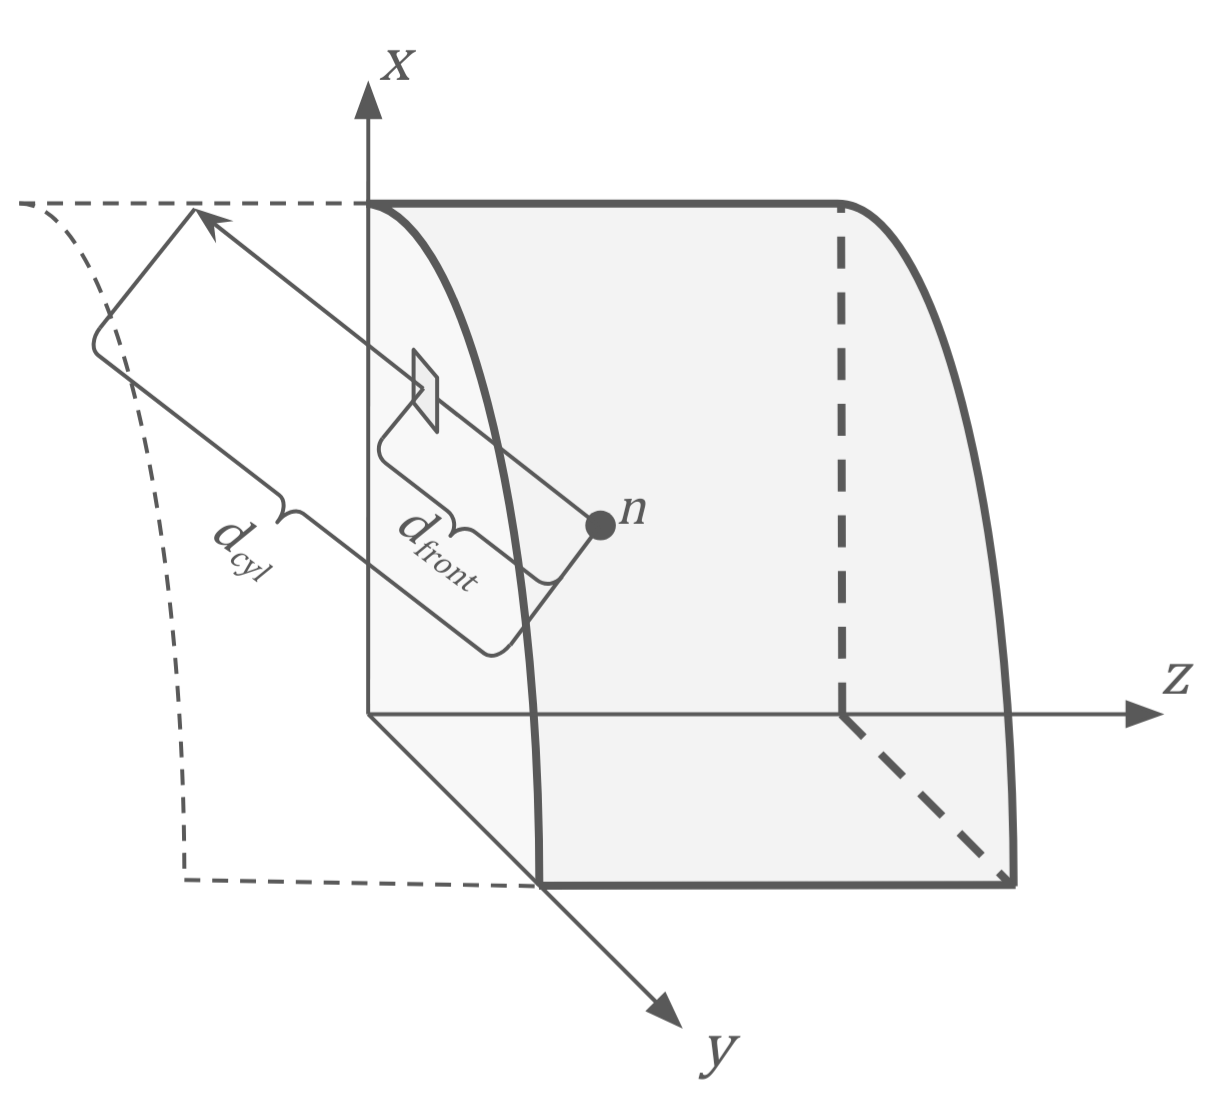
\includegraphics[width=0.75\linewidth]{Capture Yield/Figures/ms_face_intersection.png}
    \caption{Example of the face intersection scheme, resulting in $d_{front}$ being selected as the shortest face until the particle exits.}
    \label{fig:ms-face-intersection}
\end{figure}
The $d_{front}$ and $d_{back}$ terms are solved with
\begin{align}
    d_{front} &= \frac{z^k}{\Omega_{z}^{k}} \\
    d_{back} &= \frac{n - z^{k}}{\Omega^{k}_{z}}
\end{align}
while $d_{cyl}$ is is determined as
\begin{equation}
    \label{eq:cyl-intersection-distance}
    d_{cyl} = \frac{\sqrt{b^2 + ac} - b}{a}
\end{equation}
where
\begin{align}
    a &= \left( \Omega_{u}^{k} \right)^2 + \left( \Omega_{v}^{k} \right)^2\\
    b &= x^k \Omega_{u}^{k} + y^k\Omega_{v}^{k} \\
    c &= R^2 - \left( x^k \right)^2 - \left( y^k \right)^2
\end{align}

Once the $d_{front}, d_{back}, \text{ and } d_{cyl}$ distances are determined, the actual path length until escape is
\begin{equation}
    d^k =
    \begin{cases}
        \min{ \left( d_{cyl}, d_{front} \right)},   \qquad &\Omega_{w}^k < 0,\\
        d_{cyl},                                    \qquad &\Omega_{w}^k = 0, \\
        \min{ \left( d_{cyl}, d_{back} \right)},    \qquad &\Omega_{w}^k > 0,\\
    \end{cases}
\end{equation}

Next, a new set of total, capture, and elastic cross sections are sampled at energy $E^k$, which are then used to determine the sampled distance until the next collision,
\begin{equation}
    \label{eq:free-path-sampling}
    s^k = -\frac{1}{\overline{\sigma_{t} }^{k} }  \ln{\left\{
                1 - \zeta \left[ 1 - \exp{\left( \overline{\sigma_{t}}^{k} d^k \right)} \right]
    \right\}}
\end{equation}
where $\zeta$ is a randomly selected value between 0 and 1. This distance term $s^{k}$ is then used to calculate the location of the next scattering event,
\begin{equation}
    \label{eq:sampling-new-location}
    \overrightarrow{x}^{k+1} = \overrightarrow{x}^{k} + \Omega^{k}s^{k}
\end{equation}

\subsection{Sampling Energy}
\label{ssec:sampling-energy-ms}
The energy in which the neutron leaves the scattering event, i.e., $E^{k+1}$, must be determined. This introduces its own complication, as $E^{k+1}$ is dependent on the mass of the isotope it interacts with, along with its scattering angle. 

First, addressing the mass dependency. This quantity must be sampled according to each isotopes calculated scattering cross section and their given abundances, as
\begin{equation}
    w_{j} = \frac{\delta_j \sigma_{j,sc}^{k} }{\overline{\sigma_{sc}}^{k}}
\end{equation}
This quantity is then used to calculate a cumulative weight, such that
\begin{equation}
    W_j = \sum_{j} w_j
\end{equation}
This defines the window of probability for the scattering event occurring on isotope $j$ as being between $(W_{j-1}, W_{j}]$.
A random number $\zeta$ is sampled between 0 and 1, is used such that
\begin{equation}
    W_{j-1} < \zeta \leq W_{j}
\end{equation}
determines that the neutron will be sampled as scattering off a nucleus with the mass $A_j$.

Next, addressing the angle dependency. The scattering angle is assumed to be isotropic, therefore can scatter with the angle $\phi$, determined as
\begin{equation}
    \phi^k = 2\pi\zeta
\end{equation}
Therefore, the energy $E^{k+1}$ is determined as
\begin{equation}
    E^{k+1} = E^{k} \frac{A_j^{2} + 2A_{j}\cos{\left(\phi^{k}\right) + 1}}{\left( A_{j} + 1 \right)^2}
\end{equation}

\subsection{Sampling Direction}
\label{ssec:sampling-direction}
The final component of determining the new parameters of a scattering event include calculating the direction the neutron is traveling, $\overrightarrow{\Omega}^{k+1}$. Similar to \autoref{sec:sampling-energy-ms}, an angle $\theta^k$ must be sampled uniformly in the range $[0,2\pi]$. However $\theta$ must be converted from center of mass scale to lab scale, where
\begin{align}
    \cos{\theta'} &= \frac{1 + A_j \cos{\left( \theta^k \right)}}{\sqrt{1 + \left( A_j\right)^2 + 2A_j\cos{\left(\theta^k \right)}}} \\
    \sin{\theta'} &= \sqrt{1 - \left( \cos{\theta'} \right)^2}
\end{align}
while $\phi=\phi'$.
Determining $\overrightarrow{\Omega}^{k+1}$ from $\overrightarrow{\Omega}^{k}$, $\phi'$, and $\theta'$ proceed according to
\begin{equation}
    \label{eq:direction-calculation-ms}
    \overrightarrow{\Omega}^{k+1} = \begin{bmatrix}
        \Omega^{k+1}_u \\[8pt]
        \Omega^{k+1}_v \\[8pt]
        \Omega^{k+1}_w
    \end{bmatrix}
    = \begin{bmatrix}
        \frac{\Omega_{u}^{k} \Omega_{v}^{k}} { \sqrt{1 - \left(\Omega_{w}^{k}\right)^2 }} &
        \frac{-\Omega_v^k} { \sqrt{1 - \left(\Omega_{w}^{k}\right)^2 }} &
        \Omega_u \\[10pt]
        \frac{\Omega_{v}^{k} \Omega_{w}^{k}} { \sqrt{1 - \left(\Omega_{w}^{k}\right)^2 }} &
        \frac{-\Omega_u^k} { \sqrt{1 - \left(\Omega_{w}^{k}\right)^2 }} &
        \Omega_v \\[10pt]
        \frac{-1} { \sqrt{1 - \left(\Omega_{w}^{k}\right)^2 }} &
        0 &
        \Omega_w
    \end{bmatrix} \times
    \begin{bmatrix}
        \sin{\theta'}\cos{\phi'} \\[8pt]
        \sin{\theta'}\sin{\phi'} \\[8pt]
        \cos{\theta'}
    \end{bmatrix}
\end{equation}
However, in the case where $\left(\Omega_w^k\right)^2 = 1$, \autoref{eq:direction-calculation-ms} cannot be used as it would divide by 0. Instead, the operation
\begin{equation}
        \overrightarrow{\Omega}^{k+1} = \begin{bmatrix}
        \Omega^{k+1}_u \\[8pt]
        \Omega^{k+1}_v \\[8pt]
        \Omega^{k+1}_w
    \end{bmatrix} = \Omega_w^k     \begin{bmatrix}
        \sin{\theta'}\cos{\phi'} \\[8pt]
        \sin{\theta'}\sin{\phi'} \\[8pt]
        \cos{\theta'}
    \end{bmatrix}
\end{equation}
is used instead. Finally, all the components required to sample the subsequent scattering event are obtained: $\overrightarrow{x}^{k+1}$, $\overrightarrow{\Omega}^{k+1}$, and $E^{k+1}$.

\subsection{Weighting Neutrons}
\label{ssec:killing-neutrons-ms}
A calculation must be made to ensure that sufficient scattering events are being accounted for, but not so many scattering events that it is too computationally expensive, or unrealistic collision events bias the yield in some way.

A weighted importance is used to determine the contribution of a particle to capture yield and when to consider the neutron sufficiently unimportant. This is the same calculation performed by default with MCNP\cite{mcnp}. 

Given the sampled distance $s^{k}$,
\begin{align}
    \label{eq:tot-frac}
    \gamma_{tot}^{k} &=  1 - \exp{ \left(-s^{k} \overline{\sigma_{t}}^{k} \right)} \\
    \label{eq:el-frac}
    \gamma_{sc}^{k} &= \gamma_{tot}^{k} \frac{\overline{\sigma_{sc}}^{k}} {\overline{\sigma_{t}}^{k}} \\
    \label{eq:cap-frac}
    \gamma_{cap}^{k} &= \gamma_{tot}^{k} \frac{\overline{\sigma_{\gamma}}^{k}}{\overline{\sigma_{t}}^{k}}
\end{align}

The neutron weight is determined as a function of the non-captured fraction. Starting out with a weight $w^{0}=1$, the weight of a surviving neutron is the product of each non-captured fraction,
\begin{equation}
    \label{eq:neutron-weight}
    w^{k} = w^{k-1}\gamma_{el}^{k}
\end{equation}

This quantity is used in two ways; first, the factor is used to determine the total number of collisions $K$ that a neutron will experience before it is no longer statistically significant. If the weight ends up less than some cutoff factor, $\varepsilon$, the total number of collisions is reached,
\begin{equation}
    \label{eq:collision-counter}
    K = \min{ \left\{ k : w^{k} \leq \varepsilon \right\}}
\end{equation}

The second purpose of the weighting factor is to determine the total probability of capture after $K$ collisions for a single neutron history. The total probability of a neutron being captured is the sum of all weighted capture events until the collision $K$. The probability that a neutron will be captured at the $k^{th}$ collision is the product of the neutron's surviving weight from the previous collision times the capture interacting fraction $\gamma_{cap}^{k}$. This is given explicitly as
\begin{equation}
    \label{eq:capture-total-prob}
     p = \sum_{k=1}^{K} w^{k-1}\gamma_{cap}^{k}
\end{equation}

\section{Calculating The Capture Correction Factor}
\label{sec:capture-correction-factor}

The two additional quantities required to calculate the capture correction factor are the energy averaged capture cross-section, $\langle \overline{\sigma_{\gamma}} \rangle$, and energy averaged capture probability, $\langle p \rangle$. These are obtained using the $p$ term from \autoref{eq:capture-total-prob}, and $\overline{\sigma_{\gamma}}^{0}$ from \autoref{eq:average-capture-cross-section}, as
\begin{equation}
    \label{eq:avg-capture-prob}
    \langle p \rangle = \frac{1}{N} \sum_{i=1}^{N} p_{i}
\end{equation}
and
\begin{equation}
    \label{eq:avg-capture-xs}
    \langle \overline{\sigma_{\gamma}} \rangle = \frac{1}{N} \sum_{i=1}^{N} \overline{\sigma_{\gamma}}^{0}_{i}
\end{equation}
where the sum is over $N$ total neutron histories. $p$ and $\overline{\sigma_{\gamma}}$ recieve the $i$ subscript to denote that their quantities refer to the $i^{th}$ neutron history.

These quantities are then used to calculate the capture correction factor,
\begin{equation}
    \label{eq:capture-correction-factor-calc}
    C_{C} = \frac{\langle p \rangle }{\langle \overline{ \sigma_{\gamma} } \rangle n}
\end{equation}
which can then be used in \autoref{eq:correction-thin-sample-approximation} to estimate the energy averaged capture yield $\langle Y \rangle$. 

It should be noted that the average capture cross section $\langle \overline{\sigma_{\gamma}} \rangle$ calculated from \autoref{eq:avg-capture-xs} and $\langle \sigma_{\gamma} \rangle$ are not necessarily the same quantity. The $\langle \overline{\sigma_{\gamma}} \rangle$ is computed via Monte Carlo simulation, while $\langle \sigma_{\gamma} \rangle$ from \autoref{eq:correction-thin-sample-approximation} is calculated analytically.

\chapter{Fitting URR Parameters}
\label{chap:fitting}
\section{M+W Bayesian Fitting}

The goal of this fitting method is to determine a set of parameters that best describes a set of experimental measurements. Given an initial parameter vector $\mathbf{U}$, each element of which has a given prior covariance $M$, we seek to find an updated parameter vector $\mathbf{U}'$ which reduces the discrepancy between theoretical predictions, $\mathbf{t}(\mathbf{U}')$, and experimental data, $\mathbf{d}$.

This is done by performing a Bayesian least-squares optimization, using a method called $M+W$. The $M+W$ method determines the parameter vector $\mathbf{U}'$ as determined as a sum between the original parameter vector $\mathbf{U}$ plus a correction term $\Delta \theta$,
\begin{equation}
    \mathbf{U}' = \mathbf{U} + \Delta \theta
\end{equation}
and the updated covariance $\mathbf{M}'$ as
\begin{equation}
    M' = \left(M^{-1} + W\right)^{-1}
\end{equation}
in which $W$ represents the "model precision". The following will describe how to obtain the $\Delta \theta$ and $W$ terms.

Starting with $n$ parameters, the prior covariance matrix $\mathbf{M}$, which is an $n\times n$ matrix. It is assumed that the parameter uncertainties are uncorrelated, such that $\mathbf{M}$ is a diagonal matrix,
\begin{equation}
    \mathbf{M} = 
\begin{bmatrix}
\sigma_{u_1}^2 & 0 & \dots & 0 \\
0 & \sigma_{u_2}^2 & \dots & 0 \\
\vdots & \vdots & \ddots & \vdots \\
0 & 0 & \dots & \sigma_{u_n}^2
\end{bmatrix}
\end{equation}

The dataset vector, $\mathbf{d}$ has $m$ unique data points, and the experimental uncertainties are represented by $\mathbf{V}$, which is an $m \times m$ matrix. Similar to $\mathbf{M}$, the uncertainties are assumed uncorrelated, and therefore is diagonal:
\begin{equation}
    \mathbf{V} = 
\begin{bmatrix}
\sigma_{d_1}^2 & 0 & \dots & 0 \\
0 & \sigma_{d_2}^2 & \dots & 0 \\
\vdots & \vdots & \ddots & \vdots \\
0 & 0 & \dots & \sigma_{d_m}^2
\end{bmatrix}
\end{equation}

The model precision matrix $W$ is determined by the equation
\begin{equation}
    W = G^T V^{-1} G
    \label{eq:w-eq}
\end{equation}
in which $G$ is the sensitivity matrix, which is an $m \times n$ matrix. This matrix is made of elements $g_{ij}$, which represent the partial derivative of the theoretical model at the $j^{th}$ data point $t_j(\mathbf{U})$,  with the $i^{th}$ parameter $u_i$, or
\begin{equation}
    g_{ij} = \frac{\partial t_j(\mathbf{U})}{\partial u_i}
\end{equation}

Expanding Equation \ref{eq:w-eq} to solve for each element of $W$, then the element $w_{ik}$ is solved as
\begin{equation}
    w_{ik} = \sum_{j} \frac{1}{\sigma_{d_j}^2}\frac{\partial t_j(\mathbf{U})}{\partial u_i}\frac{\partial t_j(\mathbf{U})}{\partial u_k}
\end{equation}

The $\Delta \theta$ term requires an iterative solution due to the nonlinear nature of the theoretical models. At each iteration, $\Delta \theta$ is solved as the solution to the equation

\begin{equation}
    \Delta \theta = (M^{-1} + W)^{-1} y
\end{equation}
in which $y$ is calculated as
\begin{equation}
    y = G^{T}V^{-1} \left[ d - t(U) + G\Delta\theta \right]
    \label{eq:y-eq}
\end{equation}

The iterative method is required due to the utilization of the $\Delta \theta$ term in Equation \ref{eq:y-eq}. This is mitigated by setting $\Delta \theta = 0$ for the first iteration, 
\begin{equation}
    y^{(0)} = G^T V^{-1}[\, d - t(U) \,]
    \label{eq:y-first}
\end{equation}
The results from Equation \ref{eq:y-first} are then used to obtain the first $\Delta \theta$ iteration, from which the full Equation \ref{eq:y-eq} can be used on each subsequent iteration.

One issue when applying this method to nuclear data is that the uncertainties and sensitivities of the parameters can vary significantly in magnitude. In order to address this, the data is normalized by a scaling matrix $S$, in which its elements are defined as
\begin{equation}
    S_{ii} = \frac{1}{\sqrt{(M^{-1} + W)_{ii}}}
\end{equation}
This scaling is then applied to $(M^{-1} + W)$ to produce the normalized matrix $\widetilde{M}$, with
\begin{equation}
    \widetilde{M} = S (M^{-1} + W) S
\end{equation}

The elements of $\widetilde{M}$ are given as
\begin{equation}
\widetilde{M}_{ij} = \frac{(M^{-1} + W)_{ij}}{\sqrt{(M^{-1} + W)_{ii}(M^{-1} + W)_{jj}}}
\end{equation}
The numerical values of $\widetilde{M}$ are bounded between $[-1,1]$, while the diagonal elements are all equal to 1. This produces improved numerical behavior.

The scaled $\widetilde{M}$ is then used to determine a scaled update vector $\widetilde{z}$,
\begin{equation}
    \widetilde{z} = \widetilde{M}^{-1} (S\,y),
\end{equation}
The unscaled update parameter vector is then obtained from
\begin{equation}
    \Delta \theta = S \widetilde{z}
\end{equation}
and the unscaled updated covariance matrix is obtained via
\begin{equation}
    M' = S \widetilde{M}^{-1} S.
\end{equation}

Once a new $\mathbf{U}'$ is obtained, $W$, $y$, $G$, and $t(\mathbf{U}')$ are recalculated, and another $\Delta \theta$ is determined. This process continues until convergence, at which the final $\mathbf{U}'$ parameter vector best represents the experimental data while considering uncertainties.

\section{The Parameter Vector $\mathbf{U}$}

% \chapter{Evaluation}
% \label{chap:evaluation}
% \input{Evaluation/evaluation}

% \chapter{Conclusion}
% \label{chap:conclusion}
% \input{Conclusion/conclusion}




%\specialhead{ACKNOWLEDGMENT}
%The acknowledgment text goes here. Unlike chapter headings, 
%this heading is not numbered.

%\specialhead{ABSTRACT}
%Write your abstract here. Again, the heading does not receive a number.



%%%%%%%%%%%%%%%%%%%%%% Bibliography      %%%%%%%%%%%%%%%%%%%
\printbibliography[title=Literature Cited]


%%%%%%%%%%%%%%%%%%%%%%%  For Appendices  %%%%%%%%%%%%%%%%%%%
%\appendix    % This command is used only once!
%\addtocontents{toc}{\parindent0pt\vskip12pt APPENDICES} %toc entry, no page #

%Note the numbering of the chapter heading is changed.
%This is a sentence to take up space and look like text.
%\section{A Section Heading}
%This is how equations are numbered in an appendix:
%\begin{equation}
%x^2 + y^2 = z^2
%\end{equation} 
%
%\chapter{THIS IS ANOTHER APPENDIX}
%This is a sentence to take up space and look like text.

\end{document}